\chapter{Testing}

\section{Test Plan}

\begin{landscape}
\subsection{Original Outline Plan}

\begin{center}
	\begin{longtable}{|p{2cm}|p{3cm}|p{3cm}|p{3cm}|l}
		\hline
		\textbf{Test Series}   & \textbf{Purpose of Test Series}   & \textbf{Testing Strategy}   & \textbf{Strategy Rationale} \\ \hline
		1  & Validating names, numbers and other strings  & Bottom-up testing  & Components will be tested as they are developed \\ \hline
		2  & Check searching the database is working correctly & Bottom-up testing  & Components will be tested as they are developed \\ \hline
		3  & Check data is inserted into the database in the right locations & Bottom-up testing  & Components will be tested as they are developed \\ \hline
		4  & Check buttons and flow of control work as intented & Top-down testing  & Components will be tested when the program is finished to check buttons still retain their functionality \\ \hline
		5  & Test the GUI & Bottom-up testing  & Components will be tested as they are developed \\ \hline
	\end{longtable}
\end{center}

\subsection{Changes to Outline Plan}

\begin{center}
	\begin{longtable}{|p{2cm}|p{3cm}|p{3cm}|p{3cm}|}
		\hline
		\textbf{Test Series}   & \textbf{Purpose of Test Series}   & \textbf{Testing Strategy}   & \textbf{Strategy Rationale} \\ \hline
		1 & Validating names, numbers and other strings  & Bottom-up testing  & Components will be tested as they are developed \\ \hline
		2 & Check searching the database is working correctly & Bottom-up testing  & Components will be tested as they are developed \\ \hline
		3 & Check data is inserted into the database in the right locations & Bottom-up testing  & Components will be tested as they are developed \\ \hline
		4 & Check buttons and flow of control work as intented & Top-down testing  & Components will be tested when the program is finished to check buttons still retain their functionality \\ \hline
		5 & Test the GUI & Bottom-up testing  & Components will be tested as they are developed \\ \hline
		\rowcolor{lightgrey} 6 & Check data is deleted successfully & Bottom-up testing & Functions will be tested as they are developed \\ \hline
		\rowcolor{lightgrey} 7 & Check data is edited successfully & Bottom-up testing & Functions will be tested as they are developed \\ \hline
		\rowcolor{lightgrey} 8 & Check invoices are reported successfully & Bottom-up testing & Functions will be tested as they are developed \\ \hline
		\rowcolor{lightgrey} 9 & Test the system fulfills the design specifications & Top-down testing & Details will be tested and checked when the program is finished \\ \hline
	\end{longtable}
\end{center}

The light grey rows have been added. As my program has changed significantly from my original plan new areas of testing have been added.

\subsection{Original Detailed Plan}

\begin{center}
    \begin{longtable}{|p{1.5cm}|p{2.5cm}|p{2.5cm}|p{2cm}|p{2cm}|p{2cm}|}
        \hline
        \textbf{Test Series} & \textbf{Purpose of Test} & \textbf{Test Description} & \textbf{Test Data} & \textbf{Test Data Type (Normal/ Erroneous/ Boundary)} & \textbf{Expected Result} \\ \hline
        1.1 & Validate first or last name is likely to be correct & Check the string consists of just letters and is between 1 and 20 characters and contains no spaces & John, 12345, John19, J, John Smith & Normal, Erroneous, Erroneous, Boundary, Erroneous & Accepted, Error, Error, Accepted, Error \\ \hline
        1.2 & Validate town name is likely to be correct & Check the string consists of just letters, hyphens and spaces and is between 1 and 20 characters & Fordham, Walton-on-the-Naze, Bury St Edmunds, Soham19 & Normal, Normal, Normal, Erroneous & Accepted, Accepted, Accepted, Error \\ \hline
        1.3 & Validate street name is likely to be correct & Check the string consists of just letters, hyphens and spaces and is between 1 and 20 characters & Market Street, Feast Close, ChurchStreet19 & Normal, Normal, Erroneous & Accepted, Accepted, Error \\ \hline
        1.4 & Validate house name/number is likely to be correct & Check the string consists of just letters, hyphens and spaces and is between 1 and 20 characters OR is a number of 1 to 3 characters & Swan, 4, Swan4 & Normal, Normal, Erroneous & Accepted, Accepted, Error \\ \hline
        1.5 & Validate phone number is likely to be correct & Check the string consists of just numbers and is 12 characters & 01234, 012345678911, one two three & Erroneous, Normal, Erroneous & Error, Accepted, Error \\ \hline
        1.6 & Validate email is likely to be correct & Check the string consists of letters, ``@`` and ``.`` 1 to  30 characters & johnsmith.co.uk, johnsmith@longroad.ac.uk, johnsmithatlongroad.ac.uk & Erroneous, Normal, Erroneous & Error, Accepted, Error \\ \hline
        1.7 & Validate date of birth is likely to be correct & Check the string consists of just numbers and / and in the format DD/MM/YY & 15th November, 15/11/96, 15/11/1996, 15.11.96 & Erroneous, Normal, Erroneous, Erroneous & Error, Accepted, Error, Error \\ \hline
        1.8 & Validate date the invoice was sent is likely to be correct & Check the string consists of just numbers and / and in the format DD/MM/YY & 1st January, 01/01/11, 01/01/2011, 01.01.11 & Erroneous, Normal, Erroneous, Erroneous & Error, Accepted, Error, Error \\ \hline
        
        2.1 & Attempt to search for a member or parent & Check the entered details are likely to be valid and the returned objects should have been returned and that the search has returned all that it should have an not left some out & John, Smith, Chruch Street, 11 & Should return any John Smith that lives at 11 Church Street along with theirt other details & Only the John Smith at 11 Church Street is returned and only him of all the people that live at 11 Church Street  \\ \hline
        
        3.1 & Attempt to add a member & Check the entered details are likely to be valid and the data is added to the Member table and under the correct fields & John, Smith, Fordham, Chruch Street, 11, 01/01/01 & Should add John Smith to the Member table who lives at 11 Church Street in Fordham with the date of birth of 01/01/01  & John Smith is correctly added to the database \\ \hline
        3.2 & Attempt to add a parent & Check the entered details are likely to be valid and the data is added to the Parent table and under the correct fields & Jane, Smith, Fordham, Chruch Street, 11, janesmith@longroad.ac.uk, 012345678911 & Should add Jane Smith to the Member table who lives at 11 Church Street in Fordham with the email address janesmith@longroad.ac.uk and with the phone number 012345678911  & Jane Smith is correctly added to the database \\ \hline
        
        4.1 & Check all the buttons work & Check all buttons take you to the right page or work as inteded & Left click show member table, left click add new member, left click print invoices, right click show member  & Normal, Normal, Normal, Erroneous  & Accepted, Accepted, Accepted, Error \\ \hline
        
        5.1 & Make sure the windows can be resized if they are meant to be & Check the windows still display widgets correctly when resized or cannot be resized if they are not meant to be & Resize the main window, resize a pop up window & Should resize window, Should not resize window  & Window will resize, Window will not resize window \\ \hline
        5.2 & Make sure databases are displayed correctly & Check the data is displayed under the right fields and that all the data fits into the window at the default size & Visually confirm any added data is inserted into the right field and all fields are displayed & All columns should be displayed and data enter should go into the right column & All columns will be displayed and data entered will go into the right columns \\ \hline
        
    \end{longtable}
\end{center}


\subsection{Changes to Detailed Plan}

\begin{center}
    \begin{longtable}{|p{1.5cm}|p{2.5cm}|p{2.5cm}|p{2cm}|p{2cm}|p{2cm}|}
        \hline
        \textbf{Test Series} & \textbf{Purpose of Test} & \textbf{Test Description} & \textbf{Test Data} & \textbf{Test Data Type (Normal/ Erroneous/ Boundary)} & \textbf{Expected Result} \\ \hline
        1.1 & Validate first name is likely to be correct for adding a member & Check the string consists of just letters and is between 1 and 20 characters and contains no spaces & John, 12345, John19, J, John Smith & Normal, Erroneous, Erroneous, Boundary, Erroneous & Accepted, Error, Error, Accepted, Error \\ \hline
        1.2 & Validate last name is likely to be correct for adding a member & Check the string consists of just letters and is between 1 and 20 characters and contains no spaces & Smith, 12345, Smith19, S, John Smith & Normal, Erroneous, Erroneous, Boundary, Erroneous & Accepted, Error, Error, Accepted, Error \\ \hline
        1.3 & Validate town name is likely to be correct for adding a member & Check the string consists of just letters, hyphens and spaces and is between 1 and 20 characters & Fordham, Walton-on-the-Naze, Bury St Edmunds, Soham19 & Normal, Normal, Normal, Erroneous & Accepted, Accepted, Accepted, Error \\ \hline
        1.4 & Validate street name is likely to be correct for adding a member & Check the string consists of just letters, hyphens and spaces and is between 1 and 20 characters & Market Street, Feast Close, ChurchStreet19 & Normal, Normal, Erroneous & Accepted, Accepted, Error \\ \hline
        1.5 & Validate house name/number is likely to be correct for adding a member & Check the string consists of just letters, hyphens and spaces and is between 1 and 20 characters OR is a number of 1 to 3 characters & Swan, 4, Swan4 & Normal, Normal, Erroneous & Accepted, Accepted, Error \\ \hline
        \rowcolor{darkgrey} 1.6 & Validate date of birth is likely to be correct & Check the string consists of just numbers and / and in the format DD/MM/YY & 15th November, 15/11/96, 15/11/1996, 15.11.96 & Erroneous, Normal, Erroneous, Erroneous & Error, Accepted, Error, Error \\ \hline
        
        2.1 & Validate first name is likely to be correct for adding a parent & Check the string consists of just letters and is between 1 and 20 characters and contains no spaces & Sarah, 12345, Sarah19, S, Sarah Smith & Normal, Erroneous, Erroneous, Boundary, Erroneous & Accepted, Error, Error, Accepted, Error \\ \hline
        2.2 & Validate last name is likely to be correct for adding a parent & Check the string consists of just letters and is between 1 and 20 characters and contains no spaces & John, 12345, John19, J, John Smith & Normal, Erroneous, Erroneous, Boundary, Erroneous & Accepted, Error, Error, Accepted, Error \\ \hline
        2.3 & Validate town name is likely to be correct for adding a parent & Check the string consists of just letters, hyphens and spaces and is between 1 and 20 characters & Fordham, Walton-on-the-Naze, Bury St Edmunds, Soham19 & Normal, Normal, Normal, Erroneous & Accepted, Accepted, Accepted, Error \\ \hline
        2.4 & Validate street name is likely to be correct for adding a parent & Check the string consists of just letters, hyphens and spaces and is between 1 and 20 characters & Market Street, Feast Close, ChurchStreet19 & Normal, Normal, Erroneous & Accepted, Accepted, Error \\ \hline
        2.5 & Validate house name/number is likely to be correct for adding a parent & Check the string consists of just letters, hyphens and spaces and is between 1 and 20 characters OR is a number of 1 to 3 characters & Swan, 4, Swan4 & Normal, Normal, Erroneous & Accepted, Accepted, Error \\ \hline
        2.6 & Validate phone number is likely to be correct & Check the string consists of just numbers and is 12 characters & 01234, 012345678911, one two three & Erroneous, Normal, Erroneous & Error, Accepted, Error \\ \hline
        2.7 & Validate email is likely to be correct & Check the string consists of letters, ``@`` and ``.`` 1 to  30 characters & johnsmith.co.uk, johnsmith@longroad.ac.uk, johnsmithatlongroad.ac.uk & Erroneous, Normal, Erroneous & Error, Accepted, Error \\ \hline
        
        \rowcolor{darkgrey} 2.8 & Validate date the invoice was sent is likely to be correct & Check the string consists of just numbers and / and in the format DD/MM/YY & 1st January, 01/01/11, 01/01/2011, 01.01.11 & Erroneous, Normal, Erroneous, Erroneous & Error, Accepted, Error, Error \\ \hline
        
        3.1 & Attempt to search for a member or parent & Check the entered details are likely to be valid and the returned objects should have been returned and that the search has returned all that it should have an not left some out & John, Smith, Chruch Street, 11 & Should return any John Smith that lives at 11 Church Street along with theirt other details & Only the John Smith at 11 Church Street is returned and only him of all the people that live at 11 Church Street \\ \hline
        
        4.1 & Attempt to add a member & Check the entered details are likely to be valid and the data is added to the Member table and under the correct fields & John, Smith, Fordham, Chruch Street, 11, 01/01/01 & Should add John Smith to the Member table who lives at 11 Church Street in Fordham with the date of birth of 01/01/01  & John Smith is correctly added to the database \\ \hline
        4.2 & Attempt to add a parent & Check the entered details are likely to be valid and the data is added to the Parent table and under the correct fields & Jane, Smith, Fordham, Chruch Street, 11, janesmith@longroad.ac.uk, 012345678911 & Should add Jane Smith to the Member table who lives at 11 Church Street in Fordham with the email address janesmith@longroad.ac.uk and with the phone number 012345678911  & Jane Smith is correctly added to the database \\ \hline
        
        5.1 & Check all the buttons work & Check all buttons take you to the right page or work as inteded & Left click show member table, left click add new member, left click print invoices, right click show member  & Normal, Normal, Normal, Erroneous  & Accepted, Accepted, Accepted, Error \\ \hline
        
        6.1 & Make sure the windows can be resized if they are meant to be & Check the windows still display widgets correctly when resized or cannot be resized if they are not meant to be & Resize the main window, resize a pop up window & Should resize window, Should not resize window  & Window will resize, Window will not resize window \\ \hline
        6.2 & Make sure databases are displayed correctly & Check the data is displayed under the right fields and that all the data fits into the window at the default size & Visually confirm any added data is inserted into the right field and all fields are displayed & All columns should be displayed and data enter should go into the right column & All columns will be displayed and data entered will go into the right columns \\ \hline
        
        \rowcolor{lightgrey} 7.1 & Attempt to delete a member & Double click a row to delete. Reload program to check the entity is deleted & Double click an entity, single click an entity, double click outside of the table & Normal, Erroneous, Erroneous  & Entity should be deleted, no effect, no effect \\ \hline
        \rowcolor{lightgrey} 7.2 & Attempt to delete a parent & Double click a row to delete. Reload program to check the entity is deleted & Double click an entity, single click an entity, double click outside of the table & Normal, Erroneous, Erroneous  & Entity should be deleted, no effect, no effect \\ \hline
        
       \rowcolor{lightgrey} 8.1 & Edit a member & Single click a field and type the new data to edit. Reload program to check the entity is changed & Single click a field, double click a field, single click outside of the table & Normal, Normal, Erroneous  & Field should be changed, Field should be changed, no effect \\ \hline
       \rowcolor{lightgrey} 8.2 & Edit a parent & Single click a field and type the new data to edit. Reload program to check the entity is changed & Single click a field, double click a field, single click outside of the table & Normal, Normal, Erroneous  & Field should be changed, Field should be changed, no effect\\ \hline

       \rowcolor{lightgrey} 9.1 & Check report invoices is working & Single click report invoices button & Single click button, right click button & Normal, Erroneous  & Reports table should show, no effect \\ \hline

    \end{longtable}
\end{center}

The light grey rows have been added and the dark grey rows will ignored. As my program has changed significantly from my original plan new areas of testing have been added.

Any testing involving dates, such as in series 1.6 and 2.8, no longer need to be tested for as I now use combo boxes for adding dates and incorrect data cannot be entered.

\section{Test Data}

\subsection{Original Test Data}

\begin{center}
    \begin{longtable}{|p{2cm}|p{5cm}|p{8cm}|}
        \hline
        \textbf{Test Series} & \textbf{Test Data} & \textbf{Expected Result}\\ \hline
        1.10 & John & Field will be green \\ \hline
        1.11 & 12345 & Field will be red \\ \hline
        1.12 & John19 & Field will be red \\ \hline
        1.13 & J & Field will be green\\ \hline
        1.14 & John Smith &  Field is green\\ \hline
        
        1.20 & Fordham & Field is green \\ \hline
        1.21 & Walton-on-the-Naze & Field is green \\ \hline
        1.22 & Bury St Edmunds & Field is green \\ \hline
        1.23 & Soham19 & Field is red\\ \hline

        1.30 & Market-Street & Field is green \\ \hline
        1.31 & Feast Close & Field is green \\ \hline
        1.32 & Church Street19 & Field is red\\ \hline
        
        1.40 & Swan & Field will be green \\ \hline
        1.41 & Swan House & Field will be green \\ \hline
        1.42 & 4 & Field will be green \\ \hline
        1.43 & Swan 4 & Field will be red \\ \hline
        
        2.50 & 01234 & Field will be red \\ \hline
        2.51 & 01234567891 & Field will be green \\ \hline
        2.52 & one two three & Field will be red \\ \hline
        
        2.60 & johnsmith.co.uk & Field will be red \\ \hline
        2.61 & johnsmith@longroad.ac.uk & Field will be green \\ \hline
        2.62 & johnsmithatlongroad.ac.uk & Field will be red \\ \hline
        
        2.70 & 15th November & Field will be red \\ \hline
        2.71 & 15/11/96 & Field will be green \\ \hline
        2.72 & 15/11/1996 & Field will be red \\ \hline
        2.73 & 15.11.96 & Field will be red \\ \hline
        
        2.80 & 1st January & Field will be red \\ \hline
        2.81 & 01/01/11 & Field will be green \\ \hline
        2.82 & 01/01/2011 & Field will be red \\ \hline
        2.83 & 05.01.11 & Field will be red \\ \hline
        
        3.10 & John & Shows all entries with the first or last name containing ''John'' \\ \hline
        3.11 & Smith & Shows all entries with the first or last name containing ''Smith'' \\ \hline
        3.12 & John Smith &  Shows no entries as neither the first name or last name columns can contain spaces \\ \hline
        3.13 & 11 & Shows no entries as neither the first name or last name columns can contain numbers \\ \hline
        
        4.10 & Click Accept button & An entry will be added to the database in the Member table with the data currently in the fields above the button. The new data will be displayed immediatly \\ \hline
        
        4.20 & Click Accept button & An entry will be added to the database in the Parent table with the data currently in the fields above the button. The new data will be displayed immediatly \\ \hline
        
        5.10 & Left-click Display Member button & Displays the Member table with the ability to sort data \\ \hline
        5.11 & Left-click Add Member button & Displays the Member table with the ability to add new data \\ \hline
        5.12 & Left-click Print Invoices button & Displays the the Invoices table with the ability to select an invoice to print \\ \hline
        5.13 & Right-click Display Member button & Nothing should happen \\ \hline
        
        6.10 & Resize the main window & Resizes the main window \\ \hline
        6.11 & Resize a pop-up window & Does not resize the pop-up\\ \hline
        
        6.20 & Check data in the tables is displayed correctly & All data is under the right collumn \\ \hline

    \end{longtable}
\end{center}

The light grey rows have been added and the dark grey rows will ignored. As my program has changed significantly from my original plan new areas of testing have been added.

Any testing involving dates, such as in series 1.6 and 2.8, no longer need to be tested for as I now use combo boxes for adding dates and incorrect data cannot be entered.

\subsection{Changes to Test Data}

\begin{center}
    \begin{longtable}{|p{2cm}|p{5cm}|p{8cm}|}
        \hline
        \textbf{Test Series} & \textbf{Test Data} & \textbf{Expected Result}\\ \hline
        1.10 & John & Field will be green \\ \hline
        1.11 & 12345 & Field will be red \\ \hline
        1.12 & John19 & Field will be red \\ \hline
        1.13 & J & Field will be green\\ \hline
        1.14 & John Smith &  Field will be red\\ \hline
        
        1.20 & Smith & Field will be green \\ \hline
        1.21 & 12345 & Field will be red \\ \hline
        1.22 & Smith19 & Field will be red \\ \hline
        1.23 & S & Field will be green\\ \hline
        1.24 & John Smith &  Field will be red\\ \hline
        
        1.30 & Fordham & Field will be green \\ \hline
        1.31 & Walton-on-the-Naze & Field will be green \\ \hline
        1.32 & Bury St Edmunds & Field will be green \\ \hline
        1.33 & Soham19 & Field will be red\\ \hline

        1.40 & Market-Street & Field will be green \\ \hline
        1.41 & Feast Close & Field will be green \\ \hline
        1.42 & Church Street19 & Field will be red\\ \hline
        
        1.50 & Swan & Field will be green \\ \hline
        1.51 & Swan House & Field will be green \\ \hline
        1.52 & 4 & Field will be green \\ \hline
        1.53 & Swan 4 & Field will be green \\ \hline
        
        \rowcolor{darkgrey} 1.60 & 15th November & Field will be red \\ \hline
        \rowcolor{darkgrey} 1.61 & 15/11/96 & Field will be green \\ \hline
        \rowcolor{darkgrey} 1.62 & 15/11/1996 & Field will be red \\ \hline
        \rowcolor{darkgrey} 1.63 & 15.11.96 & Field will be red \\ \hline
        
        \rowcolor{darkgrey} 1.70 & 1st January & Field will be red \\ \hline
        \rowcolor{darkgrey} 1.71 & 01/01/11 & Field will be green \\ \hline
        \rowcolor{darkgrey} 1.72 & 01/01/2011 & Field will be red \\ \hline
        \rowcolor{darkgrey} 1.73 & 05.01.11 & Field will be red \\ \hline
        
        2.10 & Sarah & Field will be green \\ \hline
        2.11 & 12345 & Field will be red \\ \hline
        2.12 & Sarah19 & Field will be red \\ \hline
        2.13 & S & Field will be red\\ \hline
        2.14 & Sarah Smith &  Field will be red\\ \hline
        
        1.20 & Smith & Field is green \\ \hline
        1.21 & 12345 & Field is red \\ \hline
        1.22 & Smith19 & Field is red \\ \hline
        1.23 & S & Field is green\\ \hline
        1.24 & Sarah Smith &  Field will be red\\ \hline
        
        2.30 & Fordham & Field will be green \\ \hline
        2.31 & Walton-on-the-Naze & Field will be green \\ \hline
        2.32 & Bury St Edmunds & Field will be green \\ \hline
        2.33 & Soham19 & Field will be red\\ \hline

        2.40 & Market-Street & Field will be green \\ \hline
        2.41 & Feast Close & Field will be green \\ \hline
        2.42 & Church Street19 & Field will be red\\ \hline
        
        2.50 & Swan & Field will be green \\ \hline
        2.51 & Swan House & Field will be green \\ \hline
        2.52 & 4 & Field will be green \\ \hline
        2.53 & Swan 4 & Field will be green \\ \hline
        
        2.60 & 01234 & Field will be amber \\ \hline
        2.61 & 01234567891 & Field will be green \\ \hline
        2.62 & one two three & Field will be red \\ \hline
       
        2.70 & johnsmith.co.uk & Field will be red \\ \hline
        2.71 & johnsmith@longroad.ac.uk & Field will be green \\ \hline
        2.72 & johnsmithatlongroad.ac.uk & Field will be red \\ \hline
        
        3.10 & John & Shows all entries with the first or last name containing ''John'' \\ \hline
        3.11 & Smith & Shows all entries with the first or last name containing ''Smith'' \\ \hline
        3.12 & John Smith &  Shows no entries as neither the first name or last name columns can contain spaces \\ \hline
        3.13 & 11 & Shows no entries as neither the first name or last name columns can contain numbers \\ \hline
        
        4.10 & Click Accept button & An entry will be added to the database in the Member table with the data currently in the fields above the button. The new data will be displayed immediatly \\ \hline
        
        4.20 & Click Accept button & An entry will be added to the database in the Parent table with the data currently in the fields above the button. The new data will be displayed immediatly \\ \hline
        
        5.10 & Left-click Display Member button & Displays the Member table with the ability to sort data \\ \hline
        5.11 & Left-click Add Member button & Displays the Member table with the ability to add new data \\ \hline
        5.12 & Left-click Print Invoices button & Prints the selected Invoice \\ \hline
        5.13 & Right-click Display Member button & Nothing should happen \\ \hline
        
        6.10 & Resize the main window & Resizes the main window \\ \hline
        6.11 & Resize a pop-up window & Does not resize the pop-up\\ \hline
        
        6.20 & Check data in the tables is displayed correctly & All data is under the right collumn \\ \hline

       \rowcolor{lightgrey} 7.10 & Double click a member to delete & Member will be deleted and shown in the table \\ \hline
       \rowcolor{lightgrey} 7.11 & Single click a member to delete & Member will just be highlighted \\ \hline
       \rowcolor{lightgrey} 7.12 & Double click outside of the table & No effect \\ \hline

       \rowcolor{lightgrey} 7.20 & Double click a parent to delete & Parent will be deleted and shown in the table \\ \hline
       \rowcolor{lightgrey} 7.21 & Single click a parent to delete & Parent will just be highlighted \\ \hline
       \rowcolor{lightgrey} 7.22 & Double click outside of the table & No effect \\ \hline
        
       \rowcolor{lightgrey} 8.10 & Single click a field and type new data & Field will be replaced with new data \\ \hline
       \rowcolor{lightgrey} 8.11 & Double click a field and type new data & Field will be replaced with new data \\ \hline
       \rowcolor{lightgrey} 8.12 & Single click outside of the table & No effect \\ \hline
        
       \rowcolor{lightgrey} 8.20 & Single click a field and type new data & Field will be replaced with new data \\ \hline
       \rowcolor{lightgrey} 8.21 & Double click a field and type new data & Field will be replaced with new data \\ \hline
       \rowcolor{lightgrey} 8.22 & Single click outside of the table & No effect \\ \hline

       \rowcolor{lightgrey} 9.10 & Left click report invoices button & Reports table shows \\ \hline
       \rowcolor{lightgrey} 9.11 & Right click report invoices button & No effect \\ \hline

    \end{longtable}
\end{center}

\section{Annotated Samples}

\subsection{Actual Results}

\begin{center}
    \begin{longtable}{|p{2cm}|p{5cm}|p{8cm}|}
        \hline
        \textbf{Test Series} & \textbf{Test Data} & \textbf{Actual Result}\\ \hline
        1.10 & John & The field is green \\ \hline
        1.11 & 12345 &  The field is red \\ \hline
        1.12 & John19 &  The field is red \\ \hline
        1.13 & J &  The field is green \\ \hline
        1.14 & John Smith & The field is green \\ \hline
        
        1.20 & Smith &  The field is green \\ \hline
        1.21 & 12345 &   The field is red \\ \hline
        1.22 & Smith19 &  The field is red \\ \hline
        1.23 & S &  The field is green \\ \hline
        1.24 & John Smith & The field is green \\ \hline
        
        1.30 & Fordham &  The field is green \\ \hline
        1.31 & Walton-on-the-Naze &  The field is green \\ \hline
        1.32 & Bury St Edmunds &  The field is green \\ \hline
        1.33 & Soham19 &  The field is red \\ \hline

        1.40 & Market-Street &  The field is green \\ \hline
        1.41 & Feast Close & The field is green \\ \hline
        1.42 & Church Street19 & The field is red \\ \hline
        
        1.50 & Swan & The field is green \\ \hline
        1.51 & Swan House & The field is green \\ \hline
        1.52 & 4 & The field is green \\ \hline
        1.53 & Swan 4 & The field is green \\ \hline
        
        \rowcolor{darkgrey} 1.60 & 15th November &  \\ \hline
        \rowcolor{darkgrey} 1.61 & 15/11/96 & \\ \hline
        \rowcolor{darkgrey} 1.62 & 15/11/1996 &  \\ \hline
        \rowcolor{darkgrey} 1.63 & 15.11.96 & \\ \hline
        
        \rowcolor{darkgrey} 1.70 & 1st January &  \\ \hline
        \rowcolor{darkgrey} 1.71 & 01/01/11 &  \\ \hline
        \rowcolor{darkgrey} 1.72 & 01/01/2011 &  \\ \hline
        \rowcolor{darkgrey} 1.73 & 05.01.11 & \\ \hline
        
        2.10 & Sarah & The field is green \\ \hline
        2.11 & 12345 & The field is red \\ \hline
        2.12 & Sarah19 & The field is red\\ \hline
        2.13 & S & The field is green\\ \hline
        2.14 & Sarah Smith &  The field is green\\ \hline
        
        2.20 & Smith & The field is green \\ \hline
        2.21 & 12345 & The field is red \\ \hline
        2.22 & Smith19 & The field is red \\ \hline
        2.23 & S & The field is green \\ \hline
        2.24 & Sarah Smith & The field is green \\ \hline
        
        2.30 & Fordham & The field is green \\ \hline
        2.31 & Walton-on-the-Naze & The field is green \\ \hline
        2.32 & Bury St Edmunds & The field is green \\ \hline
        2.33 & Soham19 & The field is red \\ \hline

        2.40 & Market-Street & The field is green \\ \hline
        2.41 & Feast Close & The field is green \\ \hline
        2.42 & Church Street19 & The field is red \\ \hline
        
        2.50 & Swan & The field is green \\ \hline
        2.51 & Swan House & The field is green \\ \hline
        2.52 & 4 & The field is green \\ \hline
        2.53 & Swan 4 & The field is green \\ \hline
        
        2.60 & 01234 & The field is amber \\ \hline
        2.61 & 01234567891 & The field is green \\ \hline
        2.62 & one two three & The field is red \\ \hline
       
        2.70 & johnsmith.co.uk & The field is amber \\ \hline
        2.71 & johnsmith@longroad.ac.uk & The field is green \\ \hline
        2.72 & johnsmithatlongroad.ac.uk & The field is amber \\ \hline
        
        3.10 & John & The correct entities are returned \\ \hline
        3.11 & Smith & The correct entities are returned \\ \hline
        3.12 & John Smith &  No entities are returned \\ \hline
        3.13 & 11 & No entities are returned \\ \hline
        
        4.10 & Click Accept button & The entity is added \\ \hline
        
        4.20 & Click Accept button & The entity is added \\ \hline
        
        5.10 & Left-click Display Member button & The Display Member screen is shown \\ \hline
        5.11 & Left-click Add Member button & The Add Member screen is shown \\ \hline
        5.12 & Left-click Print Invoices button & Invoice can be chosen and printed \\ \hline
        5.13 & Right-click Display Member button & No effect \\ \hline
        
        6.10 & Resize the main window & The window is resizable \\ \hline
        6.11 & Resize a pop-up window & The window is resizable\\ \hline
        
        6.20 & Check data in the tables is displayed correctly & The data is displayed under the right columns \\ \hline

       \rowcolor{lightgrey} 7.10 & Double click a member to delete & Entitiy is deleted \\ \hline
       \rowcolor{lightgrey} 7.11 & Single click a member to delete & Entitiy is selected \\ \hline
       \rowcolor{lightgrey} 7.12 & Double click outside of the table & No effect \\ \hline

       \rowcolor{lightgrey} 7.20 & Double click a parent to delete & Entitiy is deleted \\ \hline
       \rowcolor{lightgrey} 7.21 & Single click a parent to delete & Entitiy is selected\\ \hline
       \rowcolor{lightgrey} 7.22 & Double click outside of the table & No effect \\ \hline
        
       \rowcolor{lightgrey} 8.10 & Single click a field and type new data & New data us inserted into field \\ \hline
       \rowcolor{lightgrey} 8.11 & Double click a field and type new data & The entity is deleted \\ \hline
       \rowcolor{lightgrey} 8.12 & Single click outside of the table & The field that was last clicked will be edited \\ \hline
        
       \rowcolor{lightgrey} 8.20 & Single click a field and type new data &  New data us inserted into field \\ \hline
       \rowcolor{lightgrey} 8.21 & Double click a field and type new data & The entity is deleted \\ \hline
       \rowcolor{lightgrey} 8.22 & Single click outside of the table & The field that was last clicked will be edited \\ \hline

       \rowcolor{lightgrey} 9.10 & Left click report invoices button & The Report Invoices screen is shown \\ \hline
       \rowcolor{lightgrey} 9.11 & Right click report invoices button & No effect \\ \hline
    \end{longtable}
\end{center}

\end{landscape}

\subsection{Evidence}

\subsubsection{Test 1.10 to 1.53} 
\begin{figure}[H]
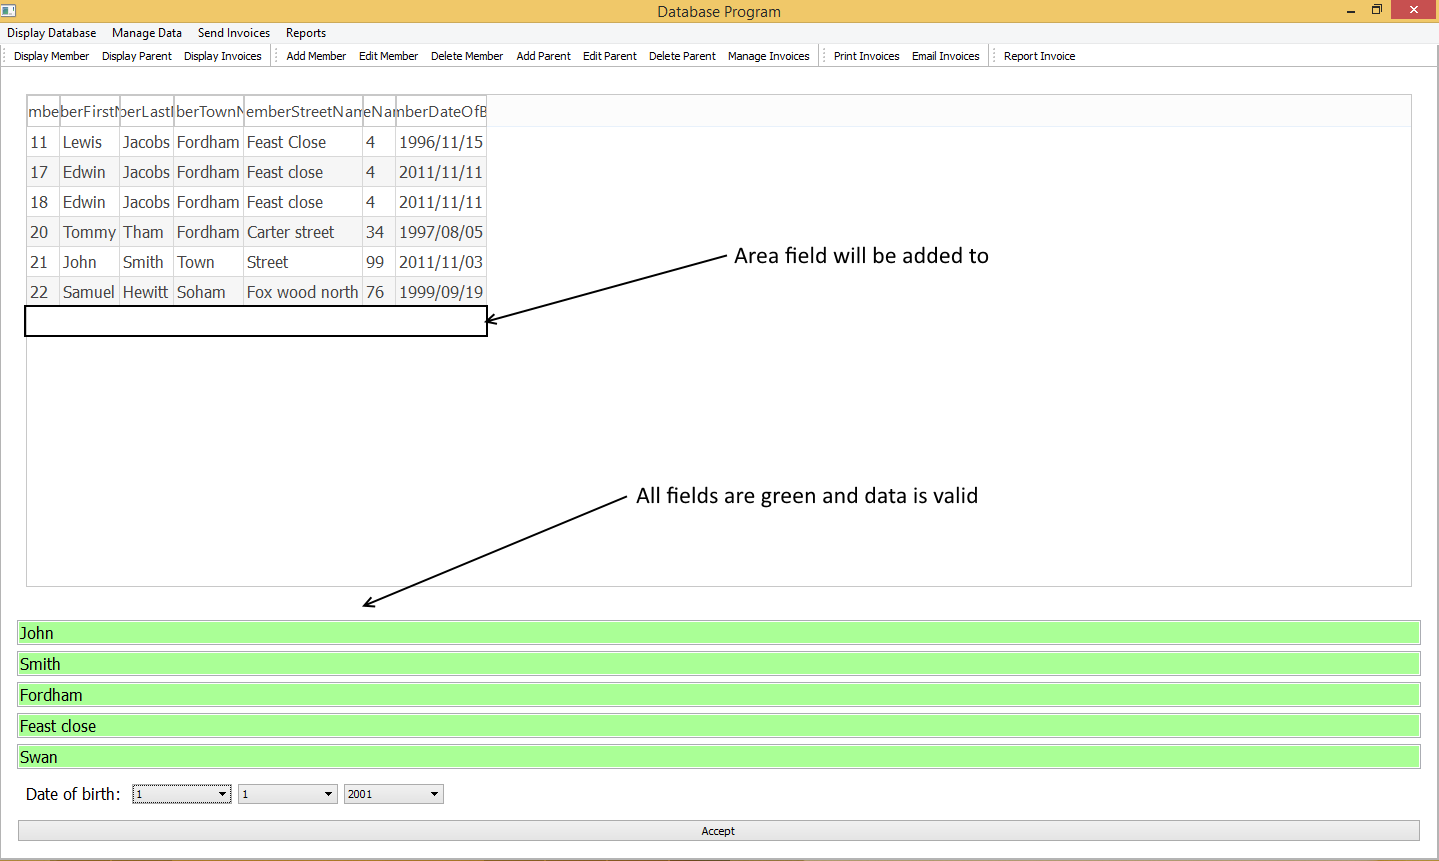
\includegraphics[width=\textwidth]{./Testing/Images/AddingMember1.png}
    \caption{Adding a member with valid fields before clicking accept} \label{fig:adding_member_1}
\end{figure}

Figure 3.3 shows the Add Member screen with valid data in all the fields before pressing the accept button

\begin{figure}[H]
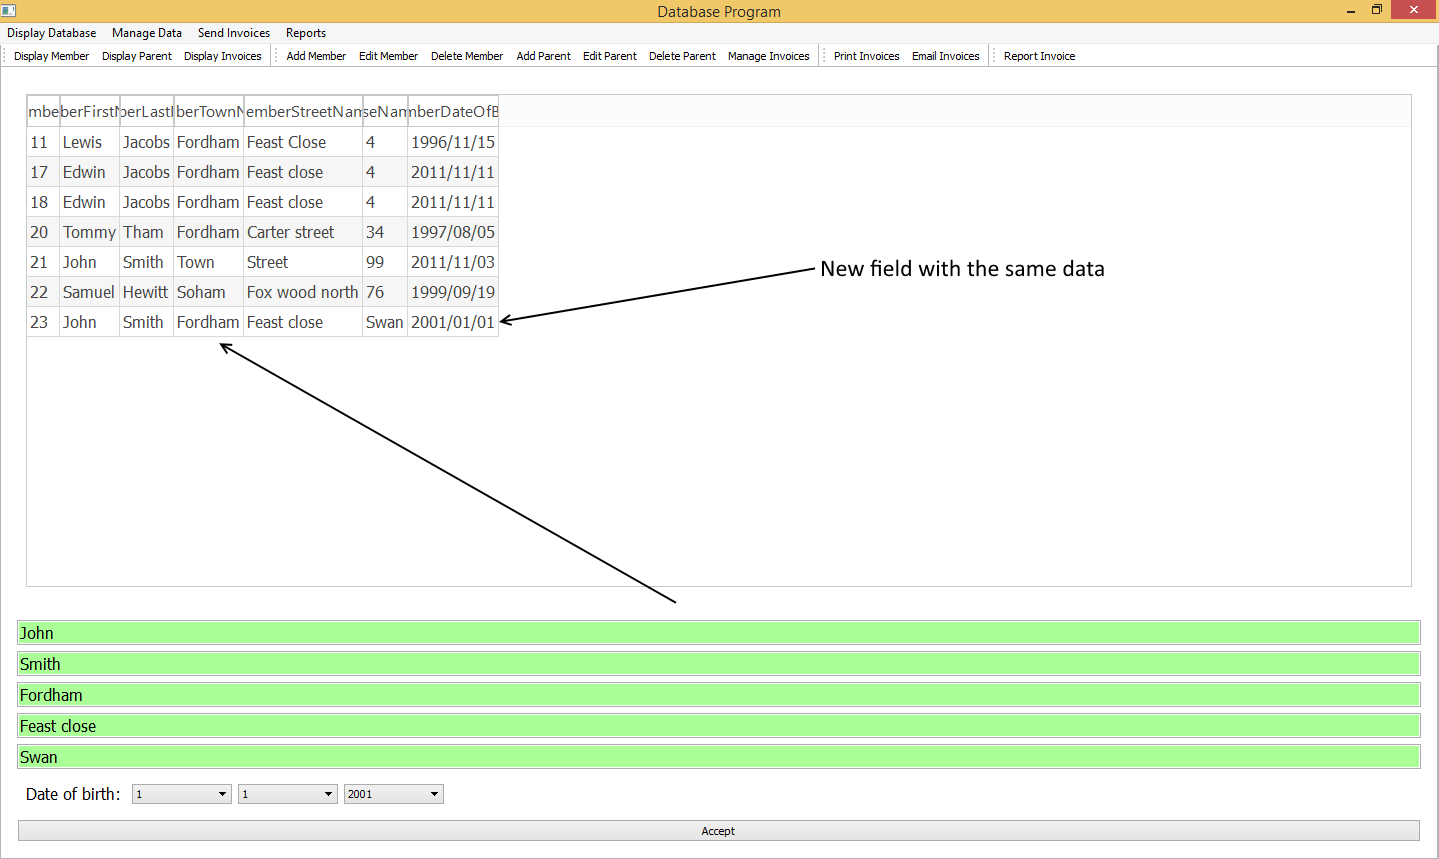
\includegraphics[width=\textwidth]{./Testing/Images/AddingMember2.png}
    \caption{Adding a member with valid fields after clicking accept} \label{fig:adding_member_2}
\end{figure}

Figure 3.4 shows the Add Member screen with valid data in all the fields after pressing the accept button. Note the presence of a new entity in the table with the same data in the correct column.

\begin{figure}[H]
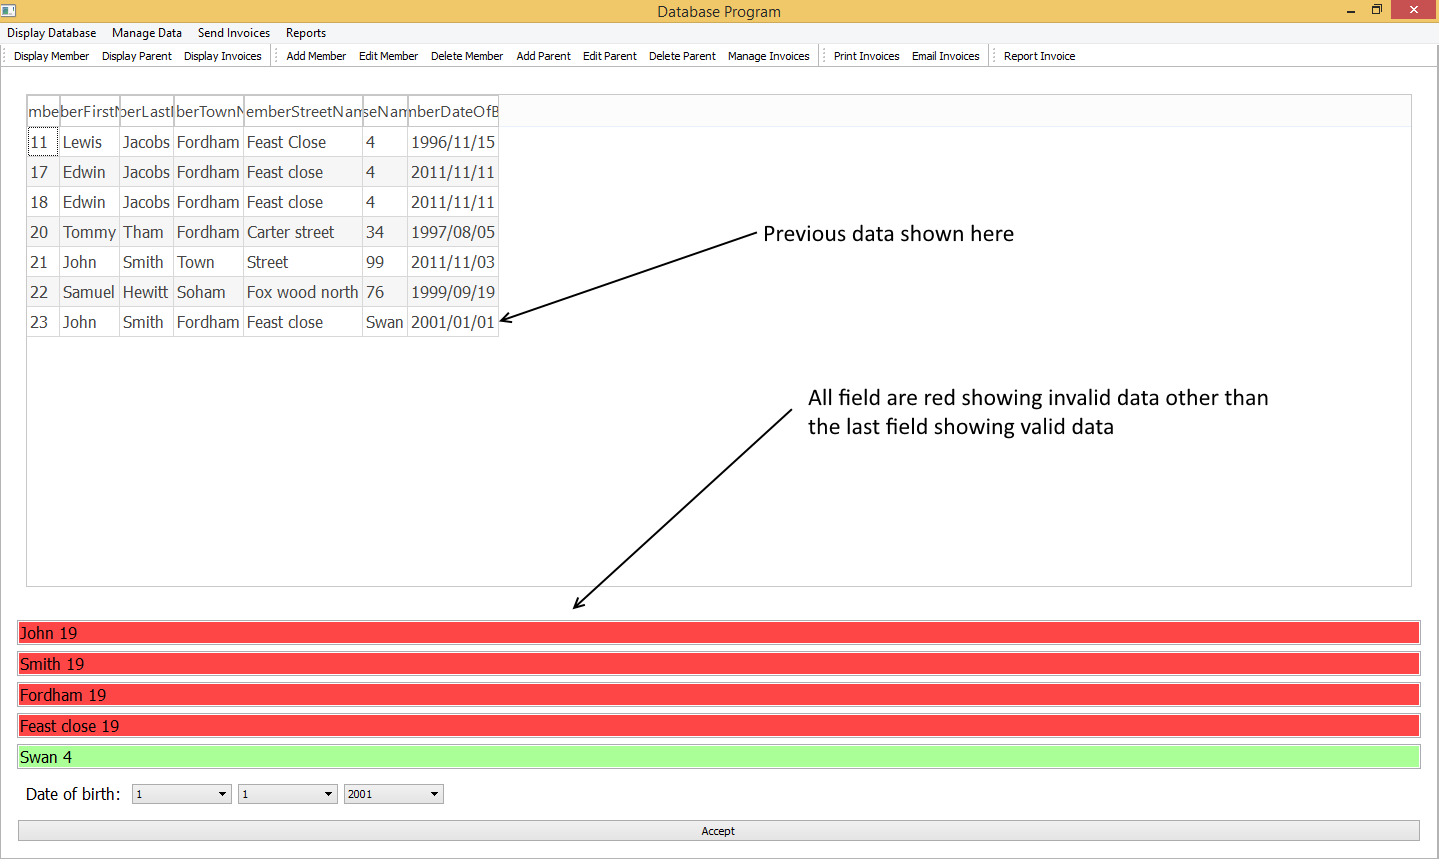
\includegraphics[width=\textwidth]{./Testing/Images/AddingMember3.png}
    \caption{Adding a member with invalid fields before clicking accept} \label{fig:adding_member_3}
\end{figure}

Figure 3.5 shows the Add Member screen with invalid data in all the fields other than Date of Birth.


\subsubsection{Test 3.10 to 3.11} 
\begin{figure}[H]
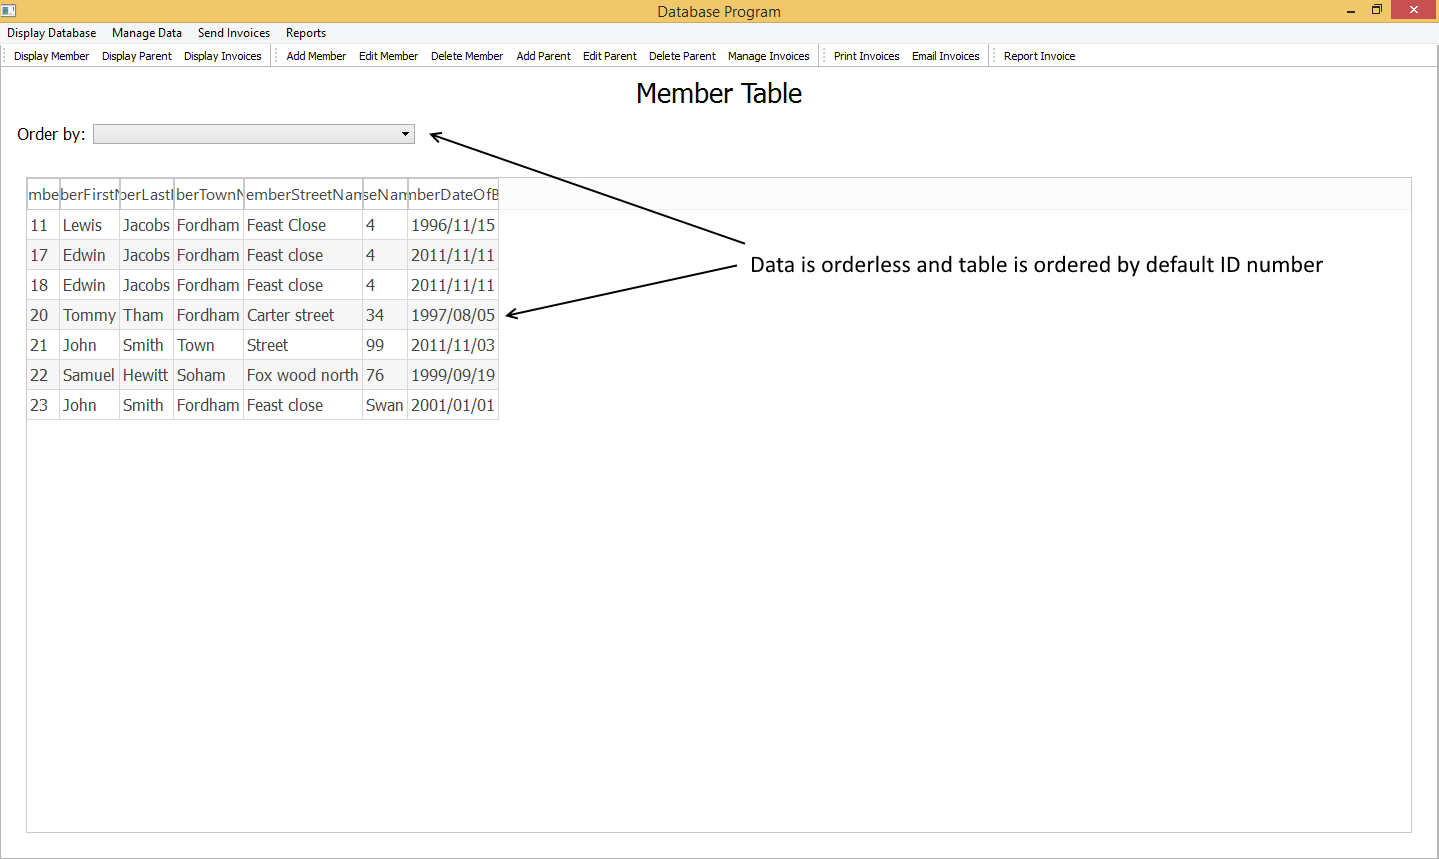
\includegraphics[width=\textwidth]{./Testing/Images/DisplayMember1.png}
    \caption{Image showing the Member table before ordering} \label{fig:display_member_1}
\end{figure}

Figure 3.1 shows the Display Member screen before sorting.

\begin{figure}[H]
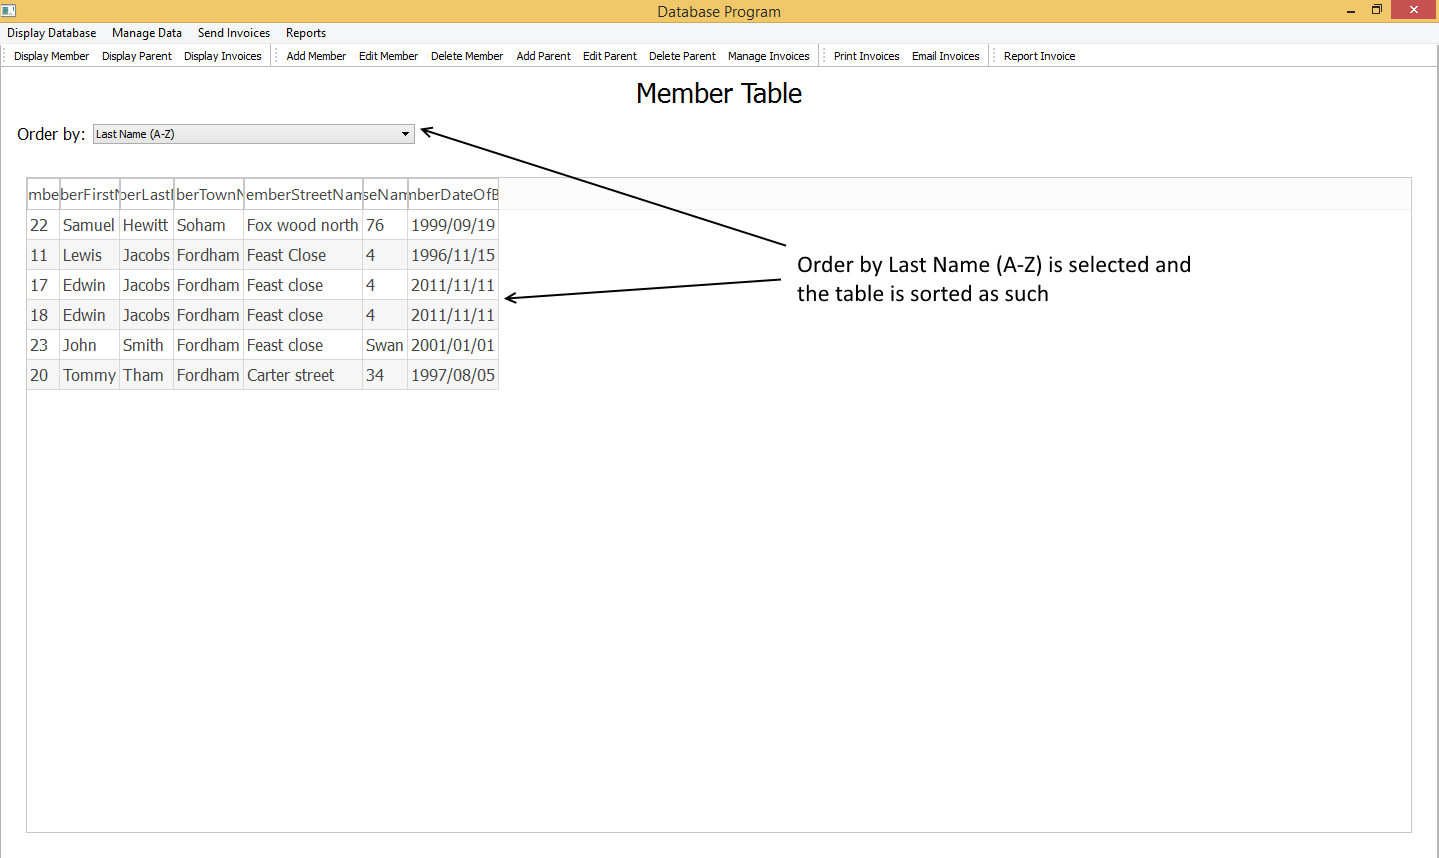
\includegraphics[width=\textwidth]{./Testing/Images/DisplayMember2.png}
    \caption{Image showing the Member table after ordering by l;ast name} \label{fig:display_member_2}
\end{figure}

Figure 3.2 shows the Display Member screen after sorting by last name from A to Z.


\subsubsection{Test 7.10 to 7.22} 
\begin{figure}[H]
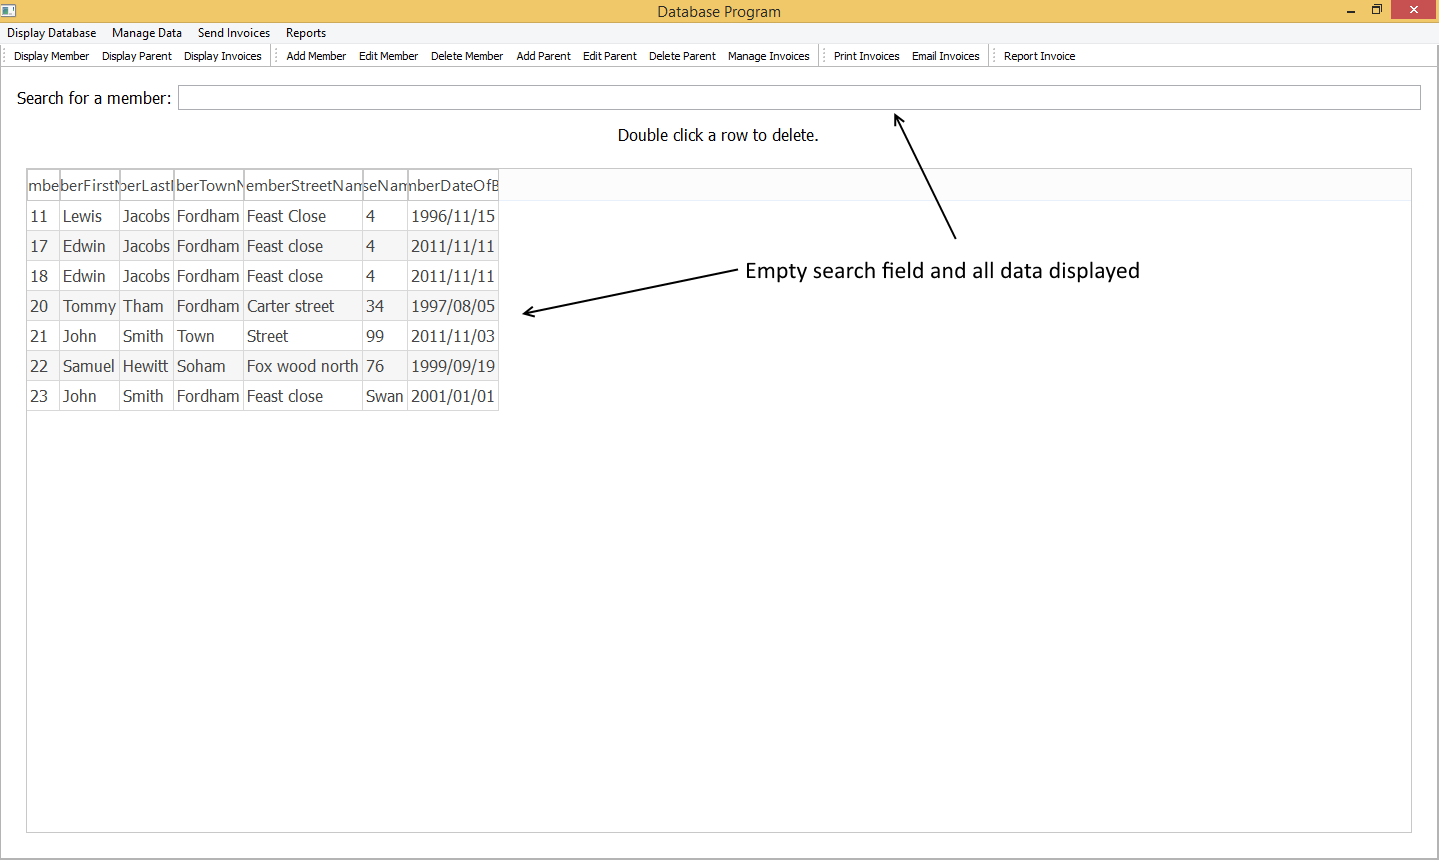
\includegraphics[width=\textwidth]{./Testing/Images/DeleteMember1.png}
    \caption{Searching and deleting a member before searching} \label{fig:delete_member_1}
\end{figure}

Figure 3.6 shows the Delete Member screen before searching for data.

\begin{figure}[H]
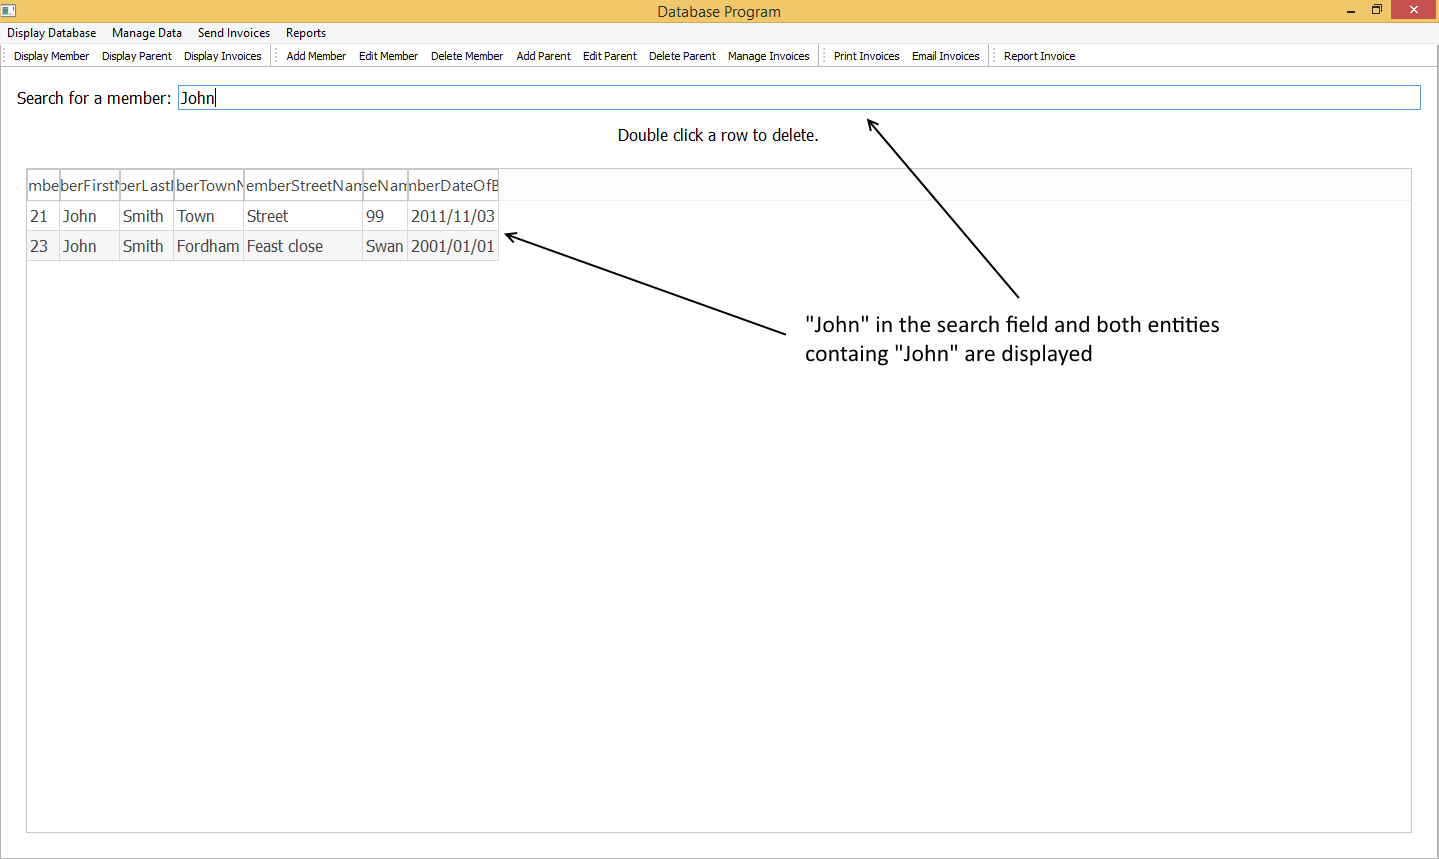
\includegraphics[width=\textwidth]{./Testing/Images/DeleteMember2.png}
    \caption{Searching and deleting a member after searching} \label{fig:delete_member_2}
\end{figure}

Figure 3.7 shows the Delete Member screen after searching for ''John''.


\begin{figure}[H]
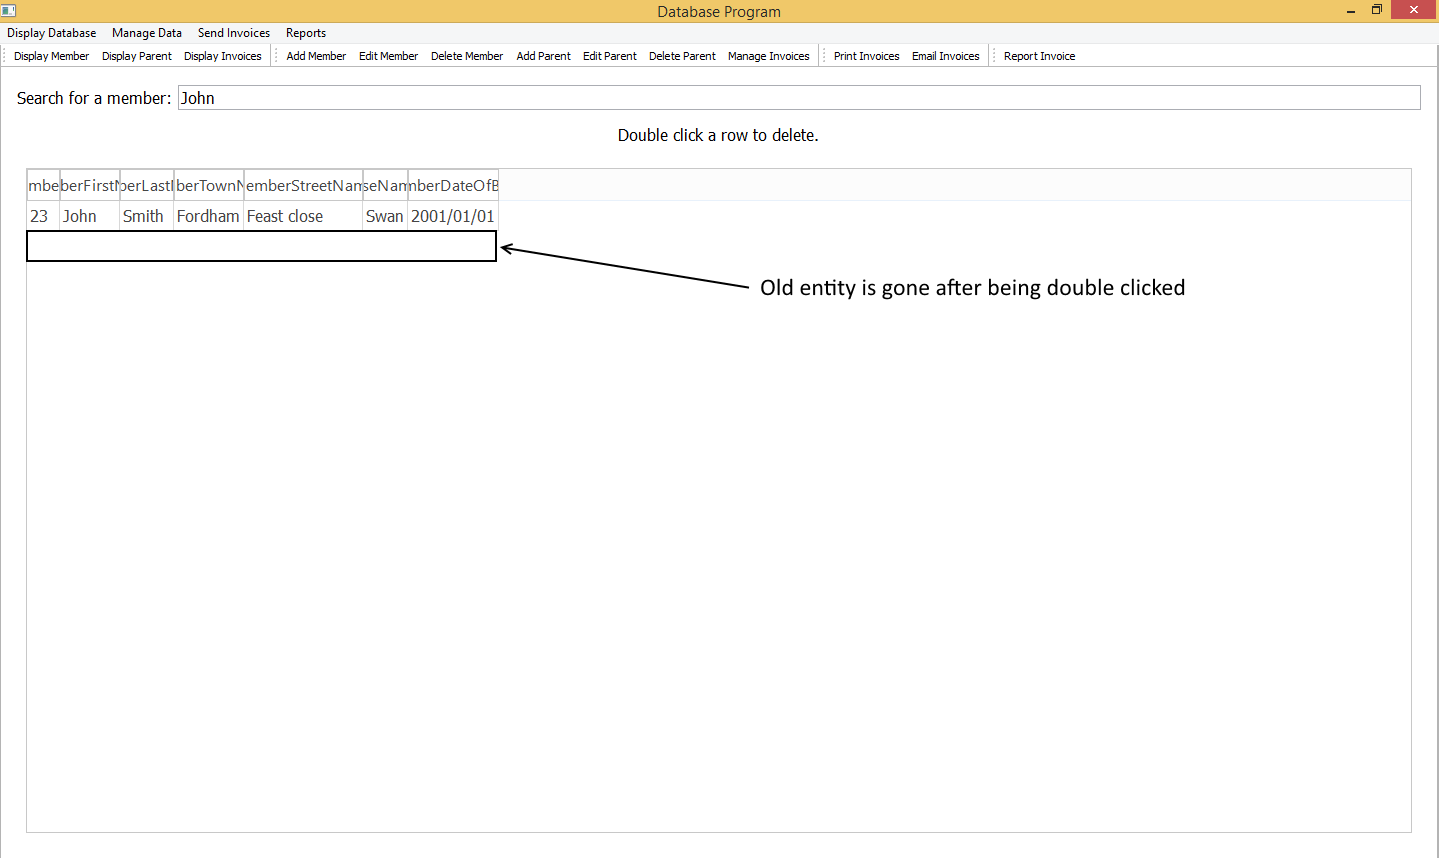
\includegraphics[width=\textwidth]{./Testing/Images/DeleteMember3.png}
    \caption{Searching and deleting a member after deleting} \label{fig:delete_member_3}
\end{figure}

Figure 3.8 shows the Delete Member screen after double clicking on the member with the ID of 21. Note that the entity has been deleted.

Showing, adding and deleting a parent all function the same way as above.


\section{Evaluation}

\subsection{Approach to Testing}
I utilised both bottom-up and top-down testing techniques. I used bottom-up testing to test individual functions of the program such as entering data into a field as the rest of the program does not affect that function. I used top-down testing for testing for testing whole areas of the program such as making sure buttons function correctly as these use multiple areas of the program.

\subsection{Problems Encountered}

\underline{Series 8.11 and 8.21} \\
I have discovered a huge error with my program, being that when a field is double clicked from anywhere, including the Display Member and Edit Member, it is deleted without warning. This is problamatic as data could easily be accidently deleted as the user is more likely to be careful when they know they need to double click to delete, and data should not be able to be deleted from those locations. This is easily fixable by adding an if statment to ensure that the current screen is either the Delete Member or Delete Parent window before deleting the data.  As additional layers of protection I could easily make a pop-up window appear for the user to decide whether they are sure they want to delete that field before the data is actually deleted.

\underline{Series 1.14, 1.24, 2.14 and 2.24} \\
Spaces could be used in the first and last name field, where they should not be allowed. Easily fixable by not including spaces in the regular expression.

\underline{Series 6.11} \\
Pop-up window are resizable when they should not be. Easily fixable by setting the resizable attribute of the windows to false.

\underline{Series 2.70 2.72} \\
Incorrect email address are displayed as amber (unfinished) when they should be displayed as incorrect (red). Work needs to be done on the regular expression and the if statements.

\subsection{Strengths of Testing}
I believe bottom-up testing to be stronger than top-down testing due to its effiecency and the speed at which testing can be got through, and if features are even just lightly tested as they are created many bugs can be fixed before going into the main testing phase, and the intricacies of the code currently being worked on are stil fresh in the coder's mind

\subsection{Weaknesses of Testing}
If I had included every possible character in my testing of validation of data to be entered then I would have spent a substantial amount of time entering every possible unicode character into each field.

\subsection{Reliability of Application}
My testing has ensured that whenever data is added into the database the user is at least alerted that the data is likely invalid. 

\subsection{Robustness of Application}
Little of my testing has been to test if there are things happening that should not be happening, for example the problem faced in series 8.11 and 8.21. I have however tested all buttons to make sure they are functioning correctly. The way that I have gone about deleting data from the database is not very robust as errors will often appear in the console although they are not visible to the user.

